
\chapter[Introdução]{Introdução}
\label{cap:introducao}



Com o intuito de reduzir a complexidade da implementação de sistemas de software, foi proposta a utilização de linguagens próximas da linguagem humana, denominadas linguagens de alto nível. Entretanto, para possibilitar a implementação de software dessa maneira, é necessário a tradução para uma linguagem que possa ser executada diretamente no \textit{hardware} \cite{aho2007compilers}.

O compilador é um sistema de \textit{software} responsável pela tradução automática de um programa em linguagem fonte de alto nível, para um programa semanticamente equivalente em uma linguagem alvo, conforme pode-se observar na Figura \ref{fig:compiler}. Deste modo, os compiladores são considerados \textit{software} básico para a computação.

\begin{figure}[!h]
\label{fig:compiler}
\centering
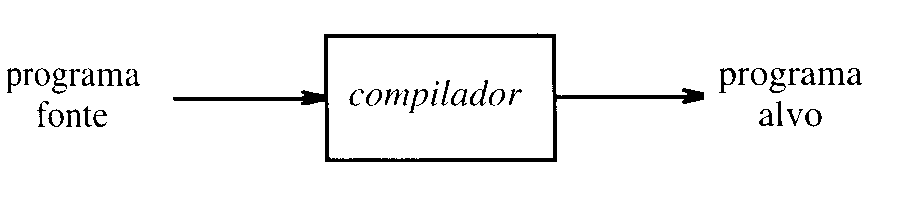
\includegraphics[width=12cm,height=12cm,keepaspectratio]{img/compiler.png}
\caption{Tradução do programa fonte para a linguagem alvo realizada pelo compilador \cite{aho2007compilers}.}
\end{figure}

O compilador é comumente dividido em módulos para reduzir a complexidade do seu processo de implementação. Essa divisão é frequentemente compreendida pelos seguintes módulos:

\begin{itemize}
    \item \textbf{Front-end (Análise)}
    \begin{itemize}
        \item \textbf{Analisador léxico}: lê o programa fonte caractere a caractere e agrupa o programa em sequências significativas denominadas lexemas. Para cada um dos lexemas é gerado um \textit{token} no formato <nome , valor>. O analisador léxico também é responsável por reconhecer e ignorar comentários e gerenciar numeração de linhas.
        \item \textbf{Analisador sintático}: recebe o fluxo de \textit{tokens} gerado pelo analisador sintático e verifica se a sequência está de acordo com a estrutura sintática da linguagem. É o núcleo do compilador.
        \item \textbf{Analisador semântico}: Utiliza a tabela de símbolos e árvore sintática para verificar se o programa-fonte atende às regras semânticas da linguagem, como regras de compatibilidade de tipos.
        \item \textbf{Gerador de código intermediário:} Código em representação intermediária em baixo nível é gerado para auxiliar a geração de código e otimização.
    \end{itemize}
    \item \textbf{Back-end (Síntese)}
    \begin{itemize}
        \item \textbf{Gerador de código:} mapeia a linguagem intermediária para a linguagem objeto. 
    \end{itemize}
\end{itemize}

A Figura \ref{fig:flow_modules} ilustra o fluxo entre os módulos do compilador:

\begin{figure}[!h]
\label{fig:flow_modules}
\centering
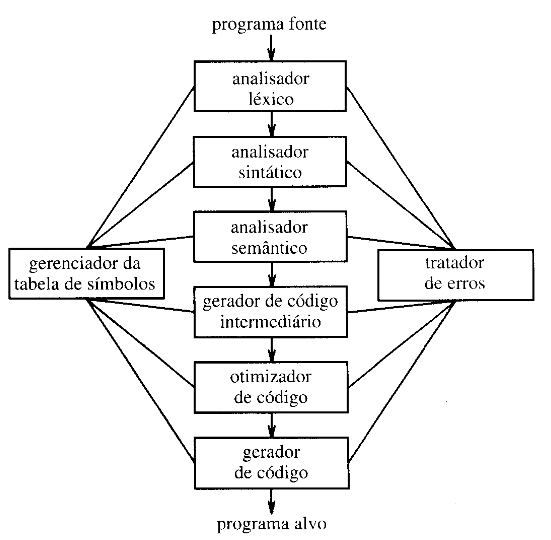
\includegraphics[width=10cm,height=10cm,keepaspectratio]{img/flow.png}
\caption{Divisão em módulos do compilador \cite{aho2007compilers}.}
\end{figure}


\section{Proposta de trabalho prático}

Foi proposto o projeto e implementação de um compilador para uma linguagem hipotética \textit{K} como trabalho prático e didático para a disciplina de Compiladores. Devido à complexidade do problema de compilação, o projeto foi dividido em quatro componentes com suas respectivas entregas:

\begin{enumerate}
    \item \label{lexico} Analisador léxico e tabela de símbolos;
    \item Analisador sintático;
    \item Analisador semântico;
    \item Gerador de código.
    
\end{enumerate}

O trabalho entregue anexo à este relatório corresponde ao analisador sintático (2). Linguagens de programação possuem regras precisas que descrevem sentenças aceitas na construção de um programa bem formado \cite{aho2007compilers}. O analisador sintático verifica se o programa-fonte submetido ao compilador está sintaticamente correto, isto é, se as ordens dos \textit{tokens} casam com as regras especificadas para a linguagem.

A organização e disposição sintática dos elementos de uma linguagem de programação é especificada por gramáticas livres de contexto. Como especificação para a linguagem \textit{K}, foi fornecida uma gramática no formato Formalismo de Backus-Naur Extendido (EBNF, do inglês \textit{Extended Backus-Naur Form}).

Deste modo, o analisador sintático recebe o fluxo de \textit{tokens} gerado pelo analisador léxico e verifica se sua ordem casa com as regras especificadas na gramática. Foi solicitado a implementação do reconhecimento das regras sintáticas especificados na gramática e identificação de erros sintáticos.

Foi proposta implementação de um analisador sintático descendente, cujo nome se origina do processo de derivação da entrada. A arvore sintática é construída de cima para baixo, produzindo uma derivação mais à esquerda para a cadeia de entrada.

O \textit{parser} recursivo descendente utiliza uma série de procedimentos recursivos, que são gerados para cada símbolo não terminal da gramática que contêm pontos de decisão de acordo com cada elemento que o respectivo símbolo não-terminal possa produzir.  

Entretanto, para que seja possível implementar este \textit{parser}, é necessário que a gramática que especifica as regras da linguagem seja classificada como LL(1). O nome indíca que a cadeia é lida da esquerda para a direita (primeiro L), é realizada um derivação mais à esquerda (segundo L) e só é necessário conhecer um único símbolo a frente para a tomada de decisões.

Para que seja classificada como LL(1), é necessário que dada gramática não contenha recursão à esquerda e produções com prefixo comum. Pode-se verificar se é possível implementar um \textit{parser} recursivo descendente para dada gramática por meio da geração de um projeto que tem como produto final a tabela do \textit{parser}. Caso não existam entradas múltiplas na tabela do \textit{parser}, a gramática é denominada LL(1). A geração da tabela do parser é realizada baseado nos conjuntos \textit{first} e \textit{follow} de cada não-terminal.

A metodologia e principais decisões tomadas nesse trabalho se encontra detalhada no Capítulo \ref{cap:metodologia}.

